\chapter{Kravspecifikation}
\label{ch:kravspecifikation}

\section{Systembeskrivelse}

\section{Funktionelle krav}
\section{Aktører}
\subsection{Aktørbeskrivelse}

% Booktabs require to add \usepackage{booktabs} to your document preamble
\begin{table}[h]
\begin{tabular}{@{}lll@{}}
\toprule
\textbf{Aktør} & \textbf{Type} & \textbf{Beskrivelse}                                          \\ \midrule
Bruger         & Primær        & Brugeren er en person, som benytter BeaconDummy eller BeaconHot \\ \midrule
BeaconBackend  &               & Web-delen af projektet                                        \\ \midrule
BeaconLib      &               & Framework                                                     \\ \midrule
BeaconDummy    &               & iPhone applikaton                                             \\ \midrule
BeaconHot      &               & iPad applikation                                              \\ \bottomrule
\end{tabular}
\end{table}

\subsection{Aktørdiagram}
\fxnote{Indsæt aktørdiagram!}
\section{Brugsscenarier}
\begin{itemize}
\item Præsentation af heat map
Brugeren bruger BeaconHot til at få en præsentation af flowet i området hvor der er opsat beacons. Denne præsentation er et heatmap og et eksempel herpå kan ses i figure \ref{fig:heatmap}. 

\begin{figure}[H]
\centering
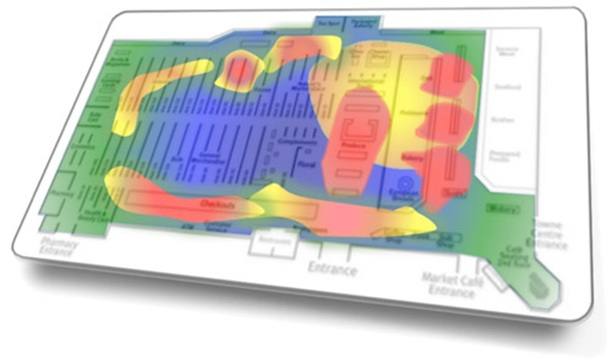
\includegraphics[width=0.6\textwidth]{billeder/heat-map}
\caption{Eksempel på hvordan en præsentation af områdeflow kan se ud}
\label{fig:heatmap}
\end{figure}

\item Scenarie 2 
\item Scenarie 3 
\item Scenarie 4 
\item Scenarie 5 
\end{itemize}